\documentclass[border=10pt]{standalone}
\usepackage{pgfplots}
\pgfplotsset{compat=1.18, trig format plots=deg}
\definecolor{v0}{HTML}{440154}\definecolor{v1}{HTML}{414487}
\definecolor{v2}{HTML}{2a788e}\definecolor{v3}{HTML}{22a884}
\definecolor{v4}{HTML}{44bf70}\definecolor{v5}{HTML}{7ad151}
\definecolor{v6}{HTML}{bddf26}\definecolor{v7}{HTML}{fde725}
\begin{document}
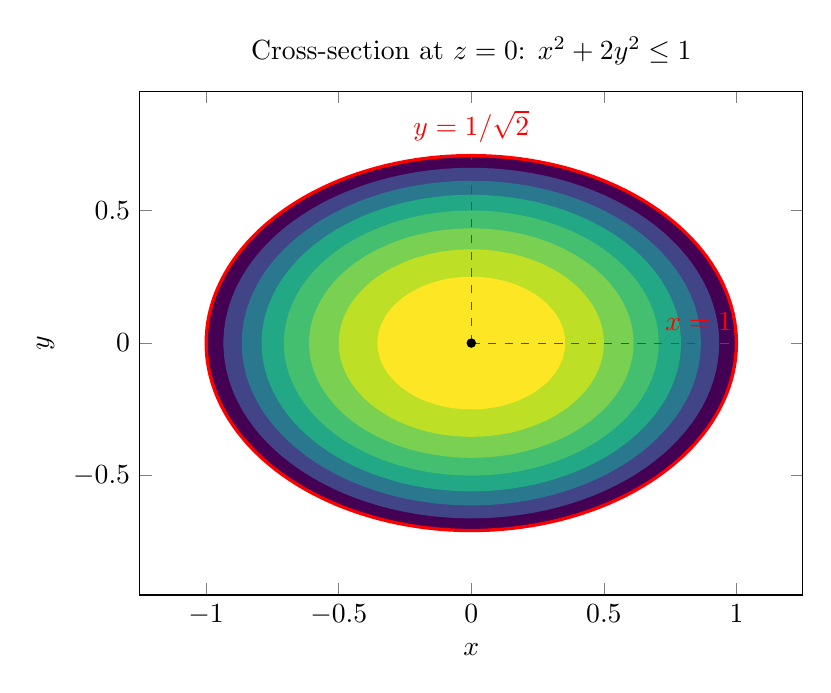
\begin{tikzpicture}
\begin{axis}[
  axis equal image,
  xlabel=$x$, ylabel=$y$,
  xmin=-1.25, xmax=1.25, ymin=-0.95, ymax=0.95,
  width=10cm, height=8cm,
  title={Cross-section at $z=0$: $x^2+2y^2\leq 1$},
]
\addplot[fill=v0, draw=none, domain=0:360, samples=120] ({1.000*cos(x)}, {0.7071*1.000*sin(x)});
\addplot[fill=v1, draw=none, domain=0:360, samples=120] ({0.935*cos(x)}, {0.7071*0.935*sin(x)});
\addplot[fill=v2, draw=none, domain=0:360, samples=120] ({0.866*cos(x)}, {0.7071*0.866*sin(x)});
\addplot[fill=v3, draw=none, domain=0:360, samples=120] ({0.791*cos(x)}, {0.7071*0.791*sin(x)});
\addplot[fill=v4, draw=none, domain=0:360, samples=120] ({0.707*cos(x)}, {0.7071*0.707*sin(x)});
\addplot[fill=v5, draw=none, domain=0:360, samples=120] ({0.612*cos(x)}, {0.7071*0.612*sin(x)});
\addplot[fill=v6, draw=none, domain=0:360, samples=120] ({0.500*cos(x)}, {0.7071*0.500*sin(x)});
\addplot[fill=v7, draw=none, domain=0:360, samples=120] ({0.354*cos(x)}, {0.7071*0.354*sin(x)});
\addplot[red, very thick, domain=0:360, samples=160] ({cos(x)}, {0.7071*sin(x)});
\addplot[red, dashed] coordinates {(0,0) (1,0)};
\addplot[red, dashed] coordinates {(0,0) (0,0.7071)};
\addplot[only marks, mark=*, mark size=1.5pt, black] coordinates {(0,0)};
\node[red, anchor=east] at (axis cs:1.02,0.08) {$x=1$};
\node[red, anchor=south] at (axis cs:0,0.72) {$y=1/\sqrt{2}$};
\end{axis}
\end{tikzpicture}
\end{document}
